%%\documentclass[preprint,12pt]{elsarticle}

%% Use the option review to obtain double line spacing
 \documentclass[preprint,review,12pt]{elsarticle}

%% Use the options 1p,twocolumn; 3p; 3p,twocolumn; 5p; or 5p,twocolumn
%% for a journal layout:
%% \documentclass[final,1p,times]{elsarticle}
%%\documentclass[final,1p,times,twocolumn]{elsarticle}
%% \documentclass[final,3p,times]{elsarticle}
%% \documentclass[final,3p,times,twocolumn]{elsarticle}
%% \documentclass[final,5p,times]{elsarticle}
%% \documentclass[final,5p,times,twocolumn]{elsarticle}

%% The graphicx package provides the includegraphics command.
\usepackage{graphicx}
%% The amssymb package provides various useful mathematical symbols
\usepackage{amssymb}
\usepackage{amsmath}
\usepackage{siunitx}
%% The amsthm package provides extended theorem environments
%% \usepackage{amsthm}

%% The lineno packages adds line numbers. Start line numbering with
%% \begin{linenumbers}, end it with \end{linenumbers}. Or switch it on
%% for the whole article with \linenumbers after \end{frontmatter}.
\usepackage{lineno}

%% natbib.sty is loaded by default. However, natbib options can be
%% provided with \biboptions{...} command. Following options are
%% valid:

%%   round  -  round parentheses are used (default)
%%   square -  square brackets are used   [option]
%%   curly  -  curly braces are used      {option}
%%   angle  -  angle brackets are used    <option>
%%   semicolon  -  multiple citations separated by semi-colon
%%   colon  - same as semicolon, an earlier confusion
%%   comma  -  separated by comma
%%   numbers-  selects numerical citations
%%   super  -  numerical citations as superscripts
%%   sort   -  sorts multiple citations according to order in ref. list
%%   sort&compress   -  like sort, but also compresses numerical citations
%%   compress - compresses without sorting
%%
%% \biboptions{comma,round}

% \biboptions{}

\journal{Journal of Mathematical Stupidity}

\begin{document}

\begin{frontmatter}

%% Title, authors and addresses

\title{Transformada de Fourier}

%% use the tnoteref command within \title for footnotes;
%% use the tnotetext command for the associated footnote;
%% use the fnref command within \author or \address for footnotes;
%% use the fntext command for the associated footnote;
%% use the corref command within \author for corresponding author footnotes;
%% use the cortext command for the associated footnote;
%% use the ead command for the email address,
%% and the form \ead[url] for the home page:
%%
%% \title{Title\tnoteref{label1}}
%% \tnotetext[label1]{}
%% \author{Name\corref{cor1}\fnref{label2}}
%% \ead{email address}
%% \ead[url]{home page}
%% \fntext[label2]{}
%% \cortext[cor1]{}
%% \address{Address\fnref{label3}}
%% \fntext[label3]{}


%% use optional labels to link authors explicitly to addresses:
%% \author[label1,label2]{<author name>}
%% \address[label1]{<address>}
%% \address[label2]{<address>}

\author{Gabriel Alexander Valdivia Medina, Giulia Alexa Naval Fernandez, Rodrigo Alonso Torres Sotomayor}

\address{Universidad Católica San Pablo, Arequipa.}

\begin{abstract}
Este trabajo está orientado en presentar la Tranformada de Fourier(TF),
explicar su funcionamiento, capacidades y versiones, así como proponer un
algoritmo en el lenguaje de programación C++ para su uso práctico. Se implementará 
una aplicación típica del algoritmo a modo de ejemplificación de lo que se puede
lograr con este. 
\end{abstract}

\begin{keyword}
Polynomial \sep solution \sep degree of a polynomial \sep linear 
\sep quadratic \sep quadratic formula \sep roots \sep cubics \sep quartics
%% keywords here, in the form: keyword \sep keyword

%% MSC codes here, in the form: \MSC code \sep code
%% or \MSC[2008] code \sep code (2000 is the default)

\end{keyword}

\end{frontmatter}

%%
%% Start line numbering here if you want
%%

%% main text
\section{La Serie de Fourier}

\[
    P(x) = a_0 + a_1x + a_2x^2 + ...  + a_ix^i
\]

It will return 0 no matter what. Since it returns 0 for any given value of $x$, it has infinite solutions.\cite{1137202}
\label{S:1}

\section{Transformada de Fourier}
La transformada de Fourier nos permite, entre muchas cosas, cambiar la forma en 
la que miramos una señal o potencia, pasando de mirar su comportamiento en 
base de tiempo a verla en base a su frecuencia.\\
Se relaciona con la Serie de Fourier, ya puede representar todas las
amplitudes de las curvas encontradas en esta serie.\\
\begin{figure}[h]
    \centering
    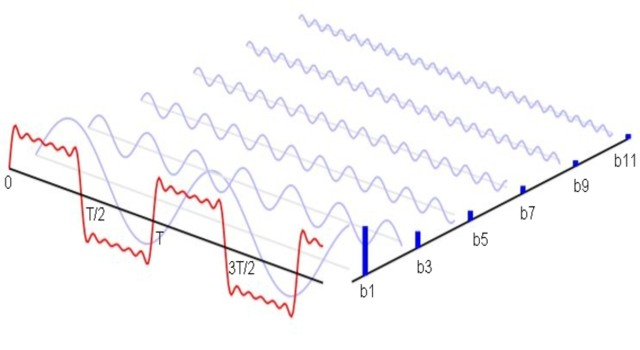
\includegraphics[scale=0.5]{Figuras/Serie-transformada.jpg}
    %%\medskip
    \\
    \small Figura1. En rojo, la señal recibida. En azul intenso, la transformada
    de Fourier. En morado, las series de Fourier. Fuente: wikimedia commons.\\
\end{figure}\\
La transformada se halla con el producto interno entre la señal recibida y una
exponencial compleja de frecuencia fija:\\
\begin{equation}
    X(f) = \int_{- \infty}^{\infty} X(t) \cdot e^{-2\pi ift} dt 
\end{equation}
Donde $X(t)$ es la señal en base tiempo definida, $X(f)$ la vista en base frecuencia
que se busca. El cambio más común es de tiempo a frecuencia, pero no es el único que la 
transformada puede manejar.\\
\subsection{Ejemplo 1}
Hallaremos la transformada de la siguiente función:\\
\begin{figure}[h]
    \centering
    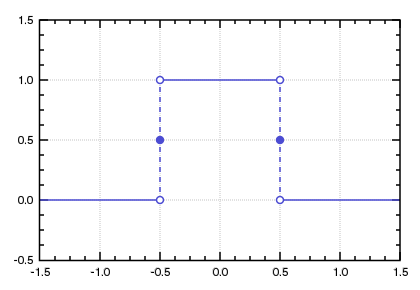
\includegraphics[scale=0.5]{Figuras/Funcion_cajon.png}
    \\
    \small Figura 2. Función rectangular, función cajón, o pulso unitario.\\
\end{figure}\\
Para hallar la transformada de una función por partes, se hallan las transformadas
de las partes por separado:\\
\[
    X(f) = \int_{- \infty}^{-0.5} rect(t) \cdot e^{-2\pi ift} dt +
    \int_{-0.5}^{0.5} rect(t) \cdot e^{-2\pi ift} dt + 
    \int_{0.5}^{\infty} rect(t) \cdot e^{-2\pi ift} dt
\]
\\
Sin embargo, dado que $rect(t)$ es igual a 0 tanto en la primera como en la
tercera parte, nos quedamos sólo con la transformada del medio.\\
\[
    X(f) = \int_{-0.5}^{0.5} 1\cdot e^{-2\pi ift} dt
\]
Desarrollamos la integral:\\
\[
    X(f) = [\frac{e^{-i2\pi ft}}{-i2\pi f}]_{-0.5}^{0.5}
\]
\[
    X(f) = \frac{e^{-i\pi f} - e^{i\pi f} }{-2\pi fi}  
\]
Por teoría de números complejos, sabemos que las funciones $sen$ y $cos$ se
relacionan con las funciones exponenciales de la forma:\\
\begin{equation}
    cos(\theta) = \frac{1}{2}(e^{+i\theta}+e^{-i\theta})
\end{equation}
\begin{equation}
    sen(\theta) = \frac{1}{2i}(e^{+i\theta}-e^{-i\theta})
\end{equation}
Entonces, pordemos acomodar nuestra ecuación para que satisfaga alguna:\\
\begin{align*}
    X(f) = \frac{-e^{-i\pi f} + e^{i\pi f}}{2i} \cdot \frac{1}{\pi f}\\
    X(f) = \frac{sen(\pi f)}{\pi f}  \\
    X(f) = sinc(\pi f)\\
\end{align*}
  

\section{Tranformada Inversa de Fourier}
\section{Algoritmo Cooley-Tukey}
\section{Algoritmo ...}
\section{Comparación de algoritmos}
\section{Aplicación Práctica: manipulación de audios usando la transformada de Fourier}
\section{Aplicación Práctica: procesado de imágenes usando la transformada de Fourier}

\section*{Apéndice}
A field is a set on which the binary operations $+$, $-$, $\times$ and $\div$ are defined.
Besides integral fields, there are other fields where polynomials will behave differently and a polynomial with finite terms and of a finite degree can also have infinite solutions.
%% The Appendices part is started with the command \appendix;
%% appendix sections are then done as normal sections
%% \appendix

%% \section{}
%% \label{}

%% References
%%
%% Following citation commands can be used in the body text:
%% Usage of \cite is as follows:
%%   \cite{key}          ==>>  [#]
%%   \cite[chap. 2]{key} ==>>  [#, chap. 2]
%%   \citet{key}         ==>>  Author [#]

%% References with bibTeX database:

\bibliographystyle{model1-num-names}
\appendix
\section*{Bibliography}
\bibliography{sample.bib}

%% Authors are advised to submit their bibtex database files. They are
%% requested to list a bibtex style file in the manuscript if they do
%% not want to use model1-num-names.bst.

%% References without bibTeX database:

% \begin{thebibliography}{00}

%% \bibitem must have the following form:
%%   \bibitem{key}...
%%

% \bibitem{}

% \end{thebibliography}


\end{document}

%%
%% End of file `elsarticle-template-1-num.tex'.